\documentclass[12pt]{scrartcl}
\usepackage[utf8]{inputenc}
\usepackage{amsmath,amssymb,amsthm}
\usepackage[croatian]{babel}
\usepackage{csquotes}
\usepackage{marvosym}
\usepackage[unicode]{hyperref}
\usepackage{thmtools}
\usepackage{tikz}
\usepackage{mathrsfs}
\usepackage{graphicx}
%\usepackage[style=numeric]{biblatex}
%\addbibresource{literatura.bib}
\usepackage{lmodern}
\usepackage[T1]{fontenc}
\usepackage{textcomp}
\usepackage[normalem]{ulem}
\usepackage{soul}
\usepackage{draftwatermark}
\SetWatermarkText{Draft}
\SetWatermarkScale{1}

\declaretheorem{teorem}
\declaretheorem[sibling=teorem]{primjer}
\declaretheorem[style=definition,sibling=teorem]{definicija}
\declaretheorem[style=remark,qed=$\|$,sibling=teorem]{napomena}
\makeatletter
\newcommand{\mypm}{\mathbin{\mathpalette\@mypm\relax}}
\newcommand{\@mypm}[2]{\ooalign{%
  \raisebox{.1\height}{$#1+$}\cr
  \smash{\raisebox{-.6\height}{$#1-$}}\cr}}
\makeatother
\DeclareMathOperator{\arctg}{arctg}
\usepackage{txfonts}
\usepackage{multirow}




\MakeOuterQuote{"}

\begin{document}


\title{Dokumentacija za bazu podataka aplikacije "Spiza"}
\author{Fran Vojković }
\date{U Visu, 16. svibnja 2020.}
\maketitle
\tableofcontents

\begin{napomena}
Javite ako nesto treba mjenjat u dokumentu.
\end{napomena}
\section{Modeliranje}

Za potrebe aplikacije uočili smo da nam je potrebno čuvati podatke o korisnicima, restoranima, nerudžbama, hrani koju restorani imaju u ponudi i povratnoj informaciji korisnika o kvaliteti. Koristimo MySQL bazu podataka. Za svakog korisnika imamo sljedeće podatke koje pamtimo: \textsf{id\_user}, \textsf{username}, \textsf{password\_hash}, \textsf{email}, \textsf{registration\_sequence}, \textsf{has\_registered}. Navedeni podaci potrebni su nam za registraciju korisnika te \textit{log in} korisnika, primarni ključ predstavlja \textbf{\textsf{id\_user}}. Svaki restoran ima sljedeće podatke: \textsf{id\_restaurant}, \textsf{password\_hash}, \textsf{email}, \textsf{registration\_sequence}, \textsf{has\_registered}, \textsf{name}, \textsf{address}, \textsf{description}. Navedeni podati potrebni su za registraciju novih restorana, \textit{log in }postojećih restorana te prikaza opisa restorana, primarni ključ je \textbf{\textsf{id\_restaurant}}. Potrebno je pohranit i podatke o jelima: \textsf{id\_food}, \textsf{name}, \textsf{description}, \textsf{waiting\_time}, \textsf{price}. Također pohranjujemo \textit{feedback} korisnika za svaku narudžbu. Kako će restorani imati mogućnost dodavanja novih jela te njihovih slika, potrebno je pohraniti \textit{upload}-ane slike na server te u bazi zapisati njihovu lokaciju. Alternativno moguće je pohraniti slike direktno u bazu no naved3eno narušava sigurnost same baze na serveru. Trebamo se odlučit za jednu opciju \textit{TBD} \ldots

\pagebreak[2]

\section{Relacijski model baze}
Na slici~\ref{fig:er} prikazan je relacijski model naše baze, boldano su označeni primarni ključevi entiteta(tablica), podcrtani su strani ključevi u entitetima(tablicama).
\begin{figure}
    \centering
    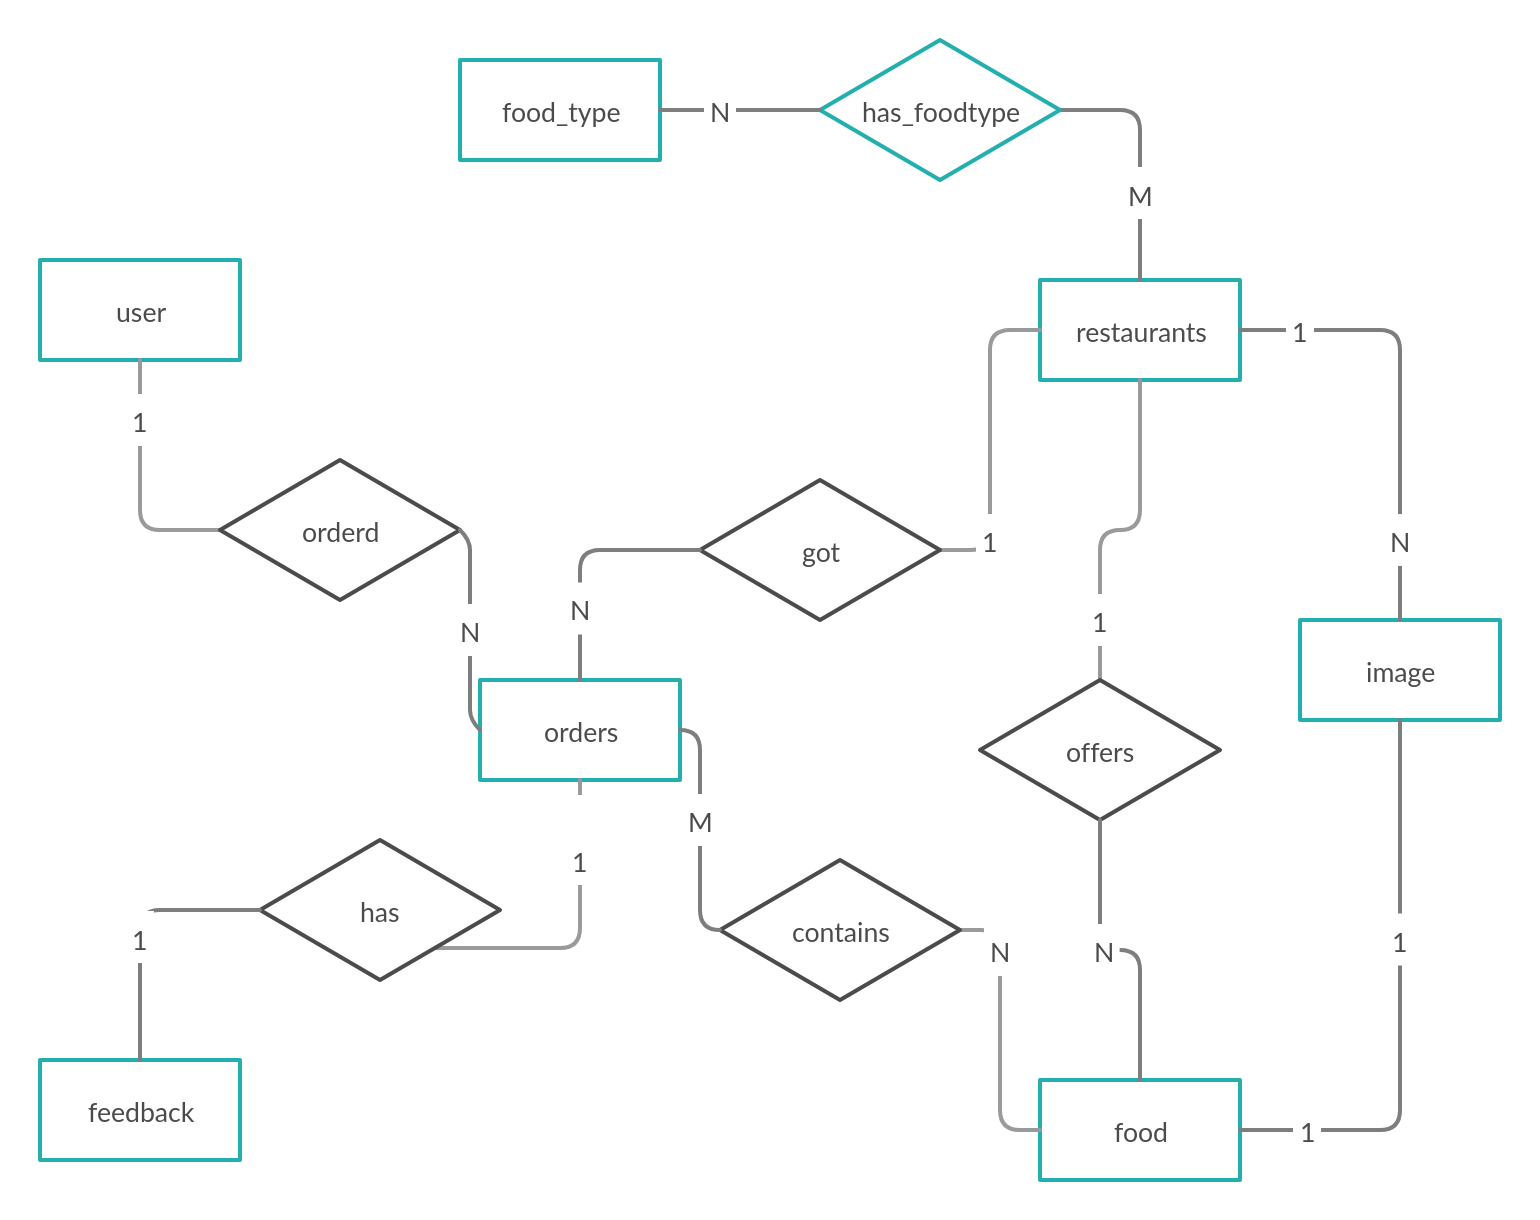
\includegraphics[width=\textwidth]{slika.png}
    \caption{ER shema modela}
    \label{fig:er}
\end{figure}

Vezu 1:N \emph{ordered} rješavamo tako da u tablicu \textsf{orders} stavimo ključ \emph{user}-a kao strani ključ. Analogno rješavamo veze 1:N \emph{offers} i \emph{got}. Veza \emph{has} je tipa 1:1 pa ubacujemo ju u orders tablicu kao atribut, a veze tipa N:M realiziramo kao posebne tablice sa primarnim ključem iz pripadajućih tablica.

Slijedi prikaz relacijskog modela:

\begin{itemize}
    \item[] \textsf{USERS (\textbf{id\_user}, username, password\_hash, email, registration\_sequence, \\has\_registered)}
    \item[] \textsf{RESTAURANTS (\textbf{id\_restaurant}, username, password\_hash, email, \\registration\_sequence, has\_registered, name, address, description)}
    \item[] \textsf{FOOD (\textbf{id\_food}, name, description, waiting\_time, price, in\_offering, \underline{id\_restaurant})}
    \item[] \textsf{FOOD\_TYPE (\textbf{id\_foodType}, name)}
    \item[] \textsf{ORDERS (\textbf{id\_order}, \underline{id\_user}, \underline{id\_restaurant}, active, order\_time, delivery\_time, price\_total, discount, note, feedback, rating, thumbs\_up, thumbs\_down)}
    \item[] \textsf{CONTAINS (\textbf{\underline{id\_order}}, \textbf{\underline{id\_food}})}
    \item[] \textsf{HAS\_FOODTYPE (\textbf{\underline{id\_foodType}}, \textbf{\underline{id\_restaurant}})}
    \item[] \textsf{IMAGE (\textbf{id\_image}, name, \underline{id\_food}, \underline{id\_restaurant}, image \emph{- vjerojatno se neće koristit- za pohranu slike})}

\end{itemize}

\pagebreak[3]

\section{Implementacija modela}

Pomoću sljedećih naredbi kreiramo bazu.

\begin{itemize}
 
    \item[] CREATE TABLE IF NOT EXISTS spiza\textunderscore users( \\
    id\_user int NOT NULL PRIMARY KEY AUTO\_INCREMENT,\\
    username varchar(50) NOT NULL,\\
    password\_hash varchar(255) NOT NULL,\\
    email varchar(50) NOT NULL,\\
    registration\_sequence varchar(20) NOT NULL,
    \\has\_registered int\\
    )
    \item[] CREATE TABLE IF NOT EXISTS spiza\_restaurants (\\
    id\_restaurant int NOT NULL PRIMARY KEY AUTO\_INCREMENT,\\
    username varchar(50) NOT NULL, \\
    password\_hash varchar(255) NOT NULL,\\
    email varchar(50) NOT NULL,\\
    registration\_sequence varchar(20) NOT NULL,\\
    has\_registered int,\\
    name varchar(50) NOT NULL,\\
    address varchar(80) NOT NULL,\\
    description varchar(50) NOT NULL\\
    )
    \item[] CREATE TABLE IF NOT EXISTS spiza\_food (\\
    id\_food int NOT NULL PRIMARY KEY AUTO\_INCREMENT,\\
    name varchar(50) NOT NULL,\\
    description varchar(200) NOT NULL,\\
    waiting\_time int NOT NULL,\\
    price decimal(6,2) NOT NULL,\\
    in\_offering tinyint NOT NULL,\\
    id\_restaurant int NOT NULL,\\
    FOREIGN KEY (id\_restaurant) REFERENCES spiza\_restaurants(id\_restaurant)
    )
    \item[] CREATE TABLE IF NOT EXISTS spiza\_food\_type (\\
    id\_foodType int NOT NULL PRIMARY KEY AUTO\_INCREMENT,\\
    name varchar(30) NOT NULL\\
    )
    \item[] CREATE TABLE IF NOT EXISTS spiza\_orders  (\\
    id\_order int NOT NULL PRIMARY KEY AUTO\_INCREMENT,\\
    id\_user int NOT NULL,\\
    id\_restaurant int NOT NULL,\\
    active tinyint NOT NULL,\\
    order\_time DATETIME NOT NULL,\\
    delivery\_time DATETIME,\\
    price\_total float,\\ 
    discount float,\\
    note varchar(50),\\
    feedback varchar(100),\\
    rating float,\\
    thumbs\_up int,\\
    thumbs\_down int, \\
    FOREIGN KEY (id\_restaurant) REFERENCES spiza\_restaurants(id\_restaurant),\\
    FOREIGN KEY (id\_user) REFERENCES spiza\textunderscore users(id\_user)\\
    )
    \item[] CREATE TABLE IF NOT EXISTS spiza\_contains (\\
    id\_order int NOT NULL,\\
    id\_food int NOT NULL,\\
    PRIMARY KEY (id\_order, id\_food),\\
    FOREIGN KEY (id\_order) REFERENCES spiza\_orders(id\_order),\\
    FOREIGN KEY (id\_food) REFERENCES spiza\_food(id\_food)\\
    )
    \item[] CREATE TABLE IF NOT EXISTS spiza\_has\_food\_type (\\
    id\_foodType int NOT NULL,\\
    id\_restaurant int NOT NULL,\\
    PRIMARY KEY (id\_foodType, id\_restaurant),\\
    FOREIGN KEY (id\_restaurant) REFERENCES spiza\_restaurants(id\_restaurant),\\
    FOREIGN KEY (id\_foodType) REFERENCES spiza\_food\_type(id\_foodType)\\
    )
    \item[] CREATE TABLE IF NOT EXISTS spiza\_image (\\
    id\_image int(11) NOT NULL PRIMARY KEY AUTO\_INCREMENT,\\
    name varchar(200) NOT NULL,\\
    image longtext,\\
    id\_food int,\\
    id\_restaurant int,\\
    FOREIGN KEY (id\_restaurant) REFERENCES spiza\_restaurants(id\_restaurant),\\
    FOREIGN KEY (id\_food) REFERENCES spiza\_food(id\_food)\\
    )
\end{itemize}

\section{To do list}
Potrebno je još dodat \st{slike restorana i jela u restoranima u bazu} te razradit sam sistem čuvanja slika na serveru, dodat za dostavljače i vjv ima još nešto. 


\end{document}
